% !TeX root = RJwrapper.tex
\title{GRAPHICS WITH R - A CROWDSOURCE BASED TRAINING INITIATIVE}
\author{by Rudradev Sengupta, Paulo R. Bargo, Bill Pikounis, Surya Mohanty, Jason Milnes, Philip Bowsher}

\maketitle

\abstract{%
Over the past decades, SAS has been a powerful tool in the data analysis
repertoire of pharmaceutical statisticians. However, the recent
development of automation capabilities based on R such as RMarkdown and
R/Shiny have created new channels to speed up creation of reports,
presentations and interactive graphics. Moreover, R helps to standardize
these processes for different phases of a drug development or submission
process \citep{Brodsky2012}. At the Johnson \& Johnson subsidiary
Janssen, we aim to improve the collective literacy in R programming
across the entire statistician community and achieve nearly 100\%
adherence by pharmaceutical statisticians and statistical programmers
over the next couple of years. In order to achieve this goal, we are
currently leveraging all types of training formats, from online
training, to in-house instructor-led seminars, to one-on-one mentoring.
Using RStudio Cloud, as a platform for internal crowd-led hands-on
workshops in particular, has been an integral part of training
statisticians/programmers to solve on-the-job problems and business
needs ranging from visualization to automated reports. In this paper, we
discuss our journey of crowdsource-based training.
}

% Any extra LaTeX you need in the preamble

\hypertarget{introduction}{%
\subsection{Introduction}\label{introduction}}

Crowdsourcing is a methodology that is becoming widely used to solve
different problems (Howe 2006). Perhaps one of the best examples of
crowdsourcing in practice is Wikipedia
(\url{https://en.wikipedia.org/wiki/Wikipedia}). In education,
crowdsourcing has been used to create content \citep{Hills2015},
assessment material development \citep{Alghamdi2015}, and practical
experience for learners \citep{Chen2014}, amongst other jobs. In this
paper, we will discuss our experience of a crowdsource-based program led
by our statisticians for the training of Janssen personnel in
visualization with R, using solely internal and open source resources.
The ``Graphics with R" initiative was crafted with the intention of
increasing scientific communication through graphical presentations,
specifically through R. Most members of clinical statistics and
statistical programming teams were not well versed in R programming, a
skill set that is becoming essential in the current landscape. The need
to acquire this new skill and the lack of time for large cohorts of team
members to engage in regular ``in-person'' classes led us to a
crowdsource-based approach where new ``on-the-job'' content was created
by more experienced volunteers from the ``crowd''. The same volunteers
supported each other and trained less experienced team members in a
``co-learning/co-teaching'' web that successfully helped us train 120
novice R programmers over a span of 8 months in a workflow that required
2-4 hours of training every other week.

\begin{figure}[h]
  \centering
  \scalebox{0.3}{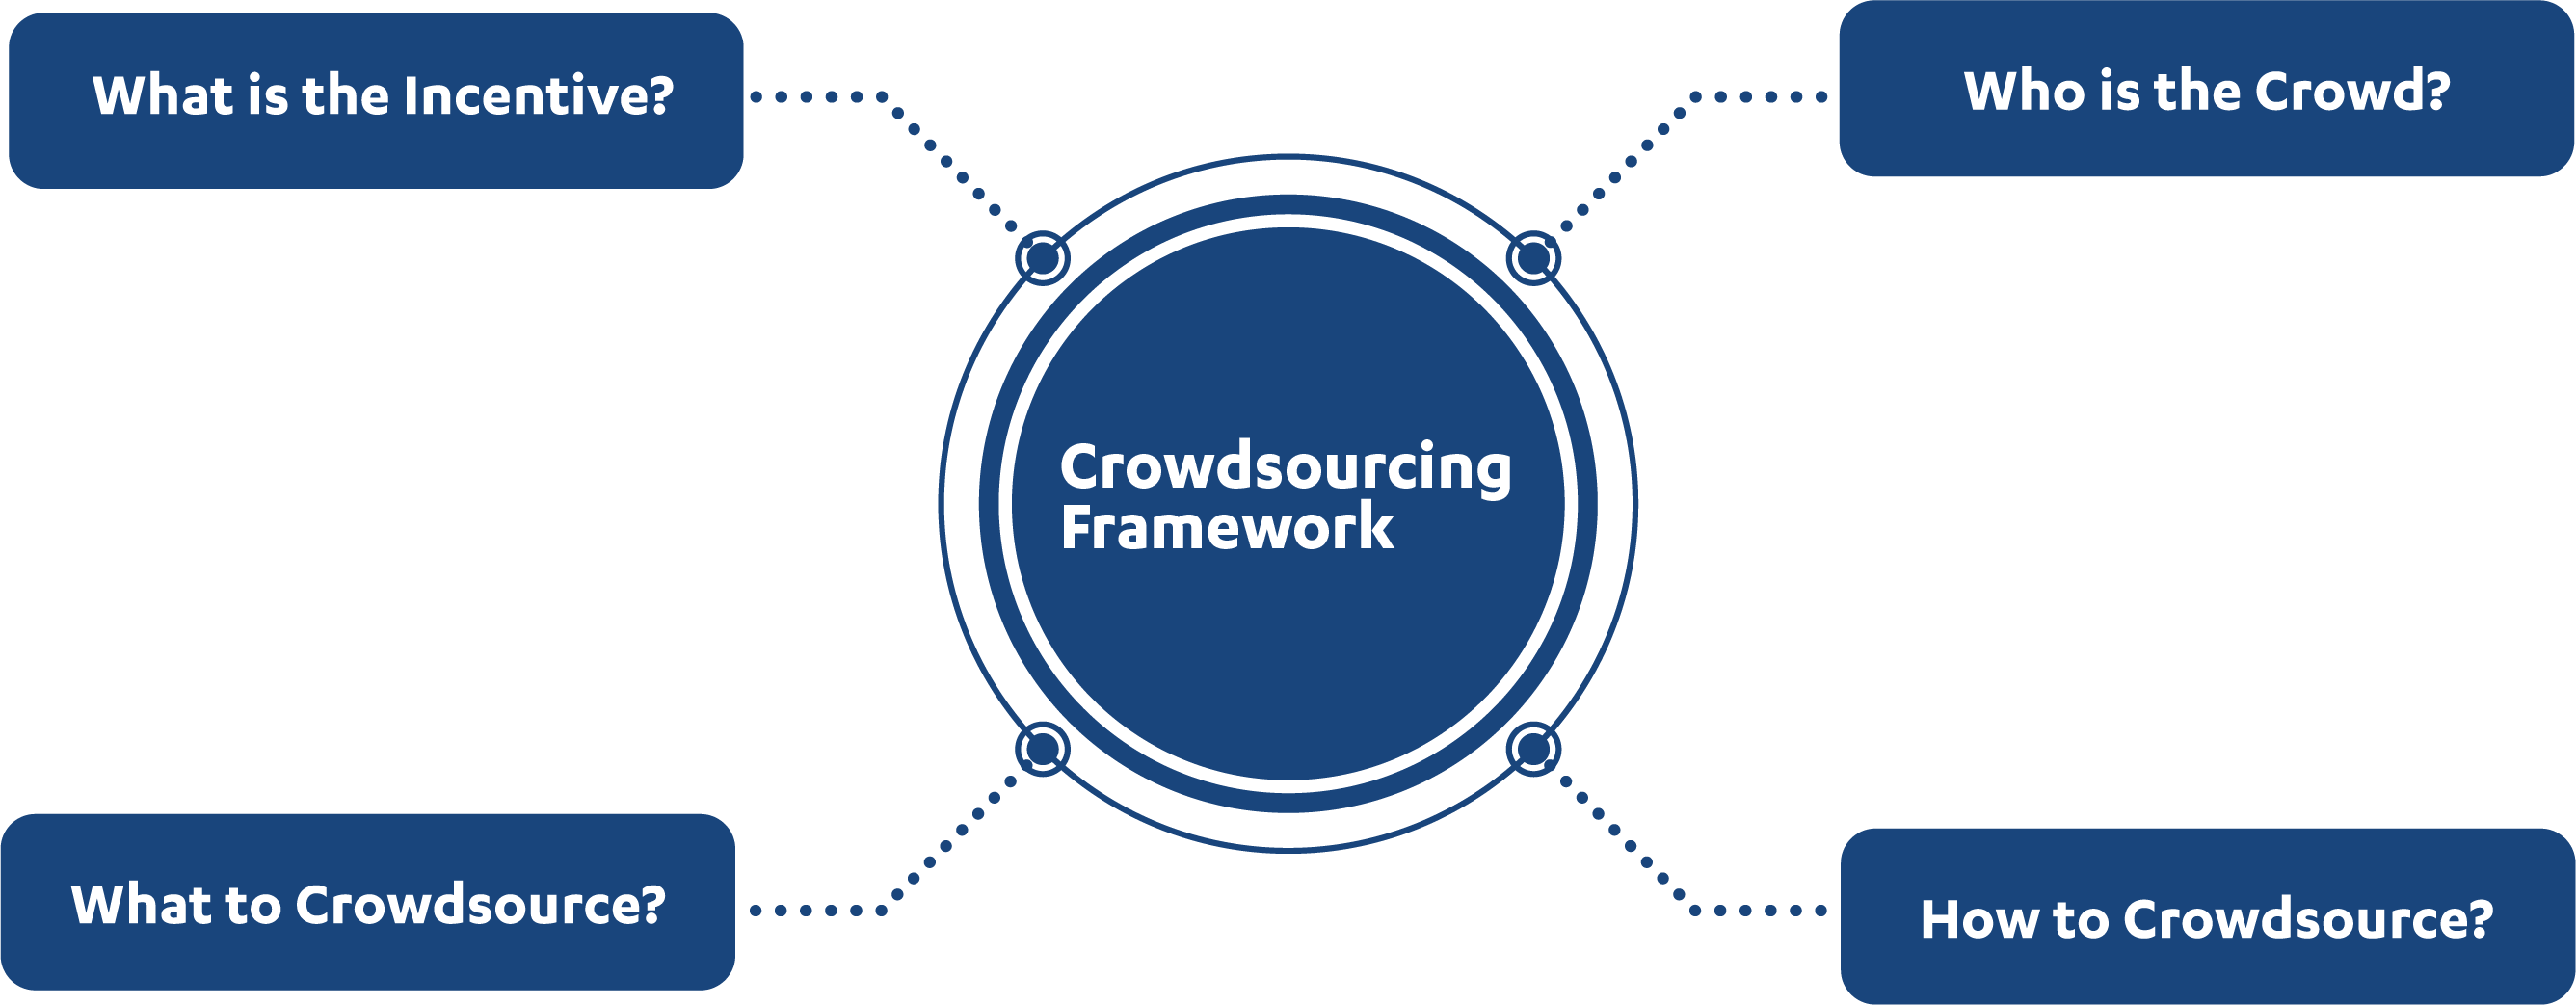
\includegraphics{figures/crowdsourceFramework3.png}}
  \caption{Crowdsourcing framework.}
  \label{figure_csfrmwrk}
\end{figure}

\hypertarget{our-approach}{%
\subsection{Our approach}\label{our-approach}}

Figure \ref{figure_csfrmwrk} asks four basic questions to setup a
crowdsource-based training framework:

\begin{itemize}
\tightlist
\item
  What is the incentive?
\item
  Who is the crowd?
\item
  What to crowdsource?
\item
  How to crowdsource?
\end{itemize}

We developed the plan for our training keeping these questions in mind.
Each of them are addressed in the next sections to explain in details
the bi-weekly approach we took to achieve our goal.

\hypertarget{what-is-the-incentive}{%
\subsubsection{What is the incentive?}\label{what-is-the-incentive}}

Crowdsourcing can be a powerful alternative method for training,
bringing in some additional benefits. One of the key aspects of
crowdsource-based training is the need for all participants to seek
knowledge as well as share it, in a co-learn/co-teach framework.
Participants with previous knowledge in R were integral part of this
initiative for the development of the curricula as well as to lead the
group meetings and become the central point of contact. An active
network was naturally created within smaller groups of people who were
already familiar with each other, which greatly facilitated the exchange
of knowledge, forming a support-group for all participants. This also
helped the leaders of the program to delegate some of their jobs and
avoid getting bombarded with questions and requests all the time on top
of their regular project work. This was particularly important in a
corporate setting because no leaders were professional educators and had
to maintain a balance between their regular jobs and the work done as
part of this training. In that sense crowdsourcing was implemented in
several levels: creation of content, hands on training, review of
performance, and creation/presentation of advanced content (tips and
tricks), with everyone contributing.

Another benefit of the process implemented was that the entire workload
was distributed over a large span of time which required a smaller
amount of work per week and a continuous engagement. Therefore the
participants had to maintain engagement and repeat their efforts in a
regular manner, which helped retaining the learning. Beyond the learning
of R, this format also helped the participants to develop soft skills as
all participants had opportunities to showcase their learning in
presentations during the regroup meetings as well as opportunities to
develop some leadership skills when leading the groups.

\hypertarget{who-is-the-crowd}{%
\subsubsection{Who is the crowd?}\label{who-is-the-crowd}}

At first, a survey was done to know the proportion of statisticians with
a background in R or who were already using R on a day-to-day basis for
regular projects. As Figure\textasciitilde{}\ref{figure_Ruser} displays,
among the respondents identified as non-clinical statisticians more than
80\% of the colleagues already had a background in R. In contrast, for
clinical statistics group, this proportion was close to one third.
Hence, the main focus audience for the training were clinical
statisticians.

\begin{figure}[htbp]
  \centering
  \scalebox{0.8}{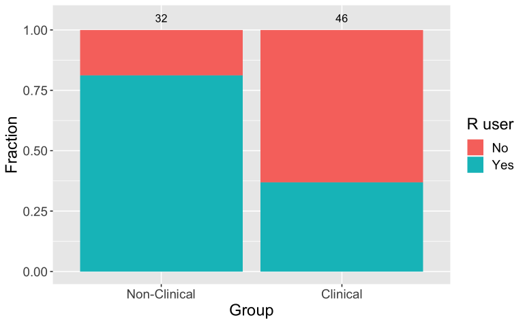
\includegraphics{figures/Ruser.png}}
  \caption{Proportion of statisticians trained in R.}
  \label{figure_Ruser}
\end{figure}

\(\vspace{0.05cm}\)

All the participants were divided into different workspaces according to
their therapeutic areas (TAs) or region they are located in. This method
of crowdsource-based training helped us to also divide the entire
workload among a group of experts who were already experienced and
regular users of R. We managed to identify approximately 30 volunteers
to help us with this initiative in different roles as described below
(refer to Figure \ref{figure_vlntrgroups}):

\begin{itemize}
\tightlist
\item
  Leads:

  \begin{itemize}
  \tightlist
  \item
    Administrate platform.
  \item
    Lead regroup sessions: US, Non-US (duplicate sessions to take care
    of the participants from different time zones across the world).
  \end{itemize}
\item
  Group Leaders:

  \begin{itemize}
  \tightlist
  \item
    Lead assignment by region/TA.
  \item
    Lead status review meeting.
  \item
    Define presenters for regroup meeting.
  \item
    Help create assignments.
  \end{itemize}
\item
  Assistants:

  \begin{itemize}
  \tightlist
  \item
    Help create assignments.
  \item
    Lead individual troubleshooting sessions.
  \item
    Present tips and tricks for visualization with R.
  \end{itemize}
\end{itemize}

\begin{figure}[htbp]
  \centering
  \scalebox{0.45}{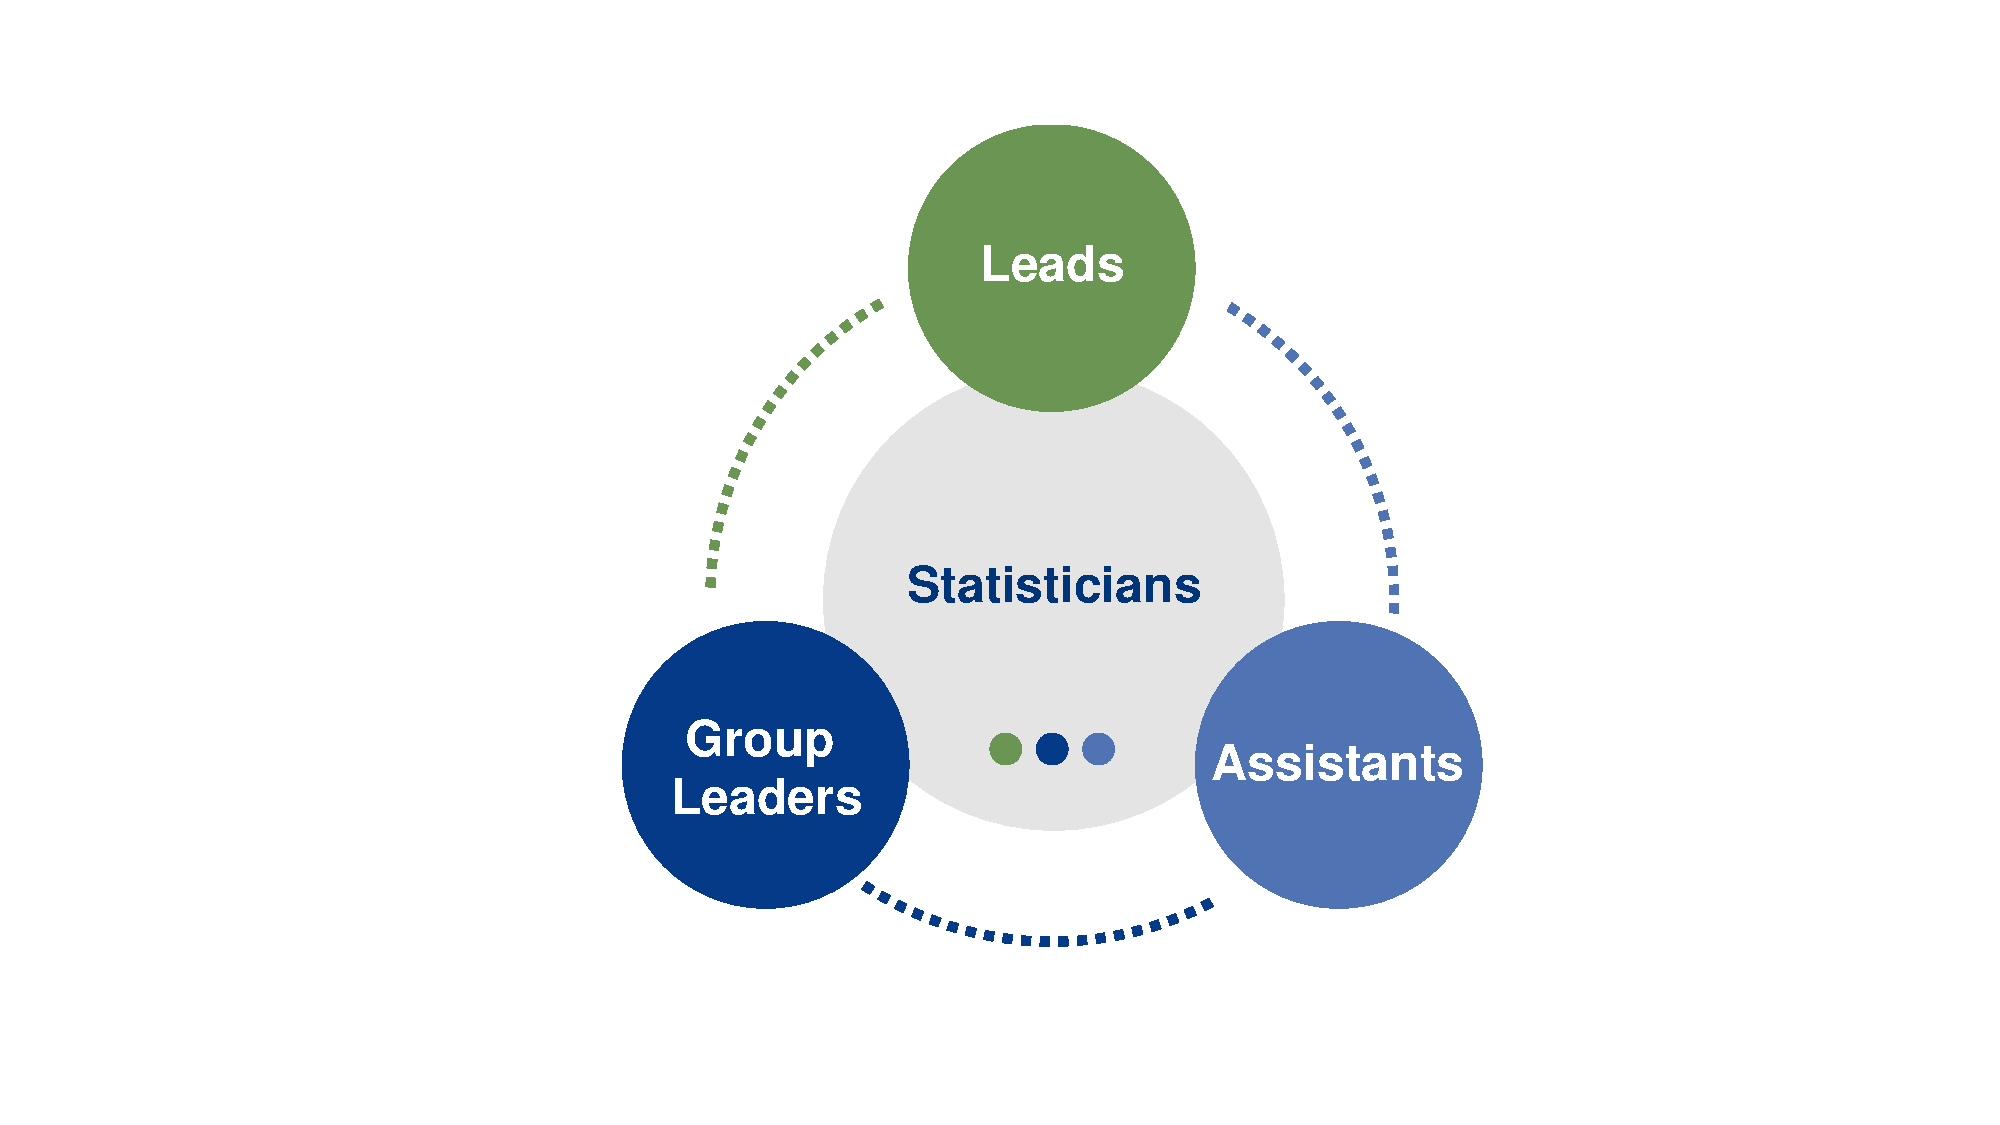
\includegraphics{figures/vlntrgroups2.pdf}}
  \caption{Division of available volunteers into different groups.}
  \label{figure_vlntrgroups}
\end{figure}

\hypertarget{what-to-crowdsource}{%
\subsubsection{What to crowdsource?}\label{what-to-crowdsource}}

The main objective of this initiative was to train statisticians to
create informative graphics by using recently developed R packages,
e.g., \texttt{ggplot2}. There were several challenges to plan this
training, e.g.~the different levels of expertise within existing
community of statisticians, difficulty to set aside time for training,
difficulty to retain knowledge with standard methods of training, etc.
These were all key items which we had to take into account before
planning this initiative. Finally, it was decided to start from simple
exercises and then keep building on top of this foundation to arrive at
more complex assignments such as animated plots, interactive plots,
etc., by the end of the course. The detailed syllabus is listed below:

\begin{itemize}
\tightlist
\item
  Assignment 1: Univariate Plots.
\item
  Assignment 2: Univariate Plots by Grouping Variable.
\item
  Assignment 3: Bivariate Plots.
\item
  Assignment 4: Linear regression.
\item
  Assignment 5: Longitudinal data analysis.
\item
  Assignment 6: Survival analysis - Kaplan-Meier, Hazard Functions, etc.
\item
  Assignment 7: ROC Curves.
\item
  Assignment 8: Forest Plots.
\item
  Assignment 9-10: RMarkdown.
\item
  Assignment 11-12: Arranging Data for Clear Communication.
\item
  Assignment 13: Tidyverse (tidyr and dplyr) and By Processing.
\item
  Assignment 14: Heatmaps.
\item
  Assignment 15: Interactive and Animated plots.
\item
  Assignment 16: Interactive Dashboards with Flexdashboard and Shiny.
\end{itemize}

\noindent \textbf{Examples}

The above syllabus was created in consultation with our team of experts
and represented typical graphics used in drug submission packages from
the different TAs. Data had to be blinded or simulated as RStudio Cloud
access did not exist within Janssen firewall. Every assignment consisted
of a dataset together with a data description file and questions related
to that particular assignment. After a few weeks, feedback was collected
from all the participants, both learners and internal expert
instructors. While initially, the first couple of assignments were
prescriptive, in desired results, it was decided to add hints and make
some questions of the assignment optional based on the feedback from the
TA leads. On one hand, it managed the workload for the beginners to gain
skills and confidence. On the other hand, interested participants could
further explore with their intellectual curiosity. The materials for all
the assignments are available
\href{https://github.com/rsengup4/GraphicsWithR}{online}.

\begin{figure}[htbp]
  \centering
  \scalebox{0.38}{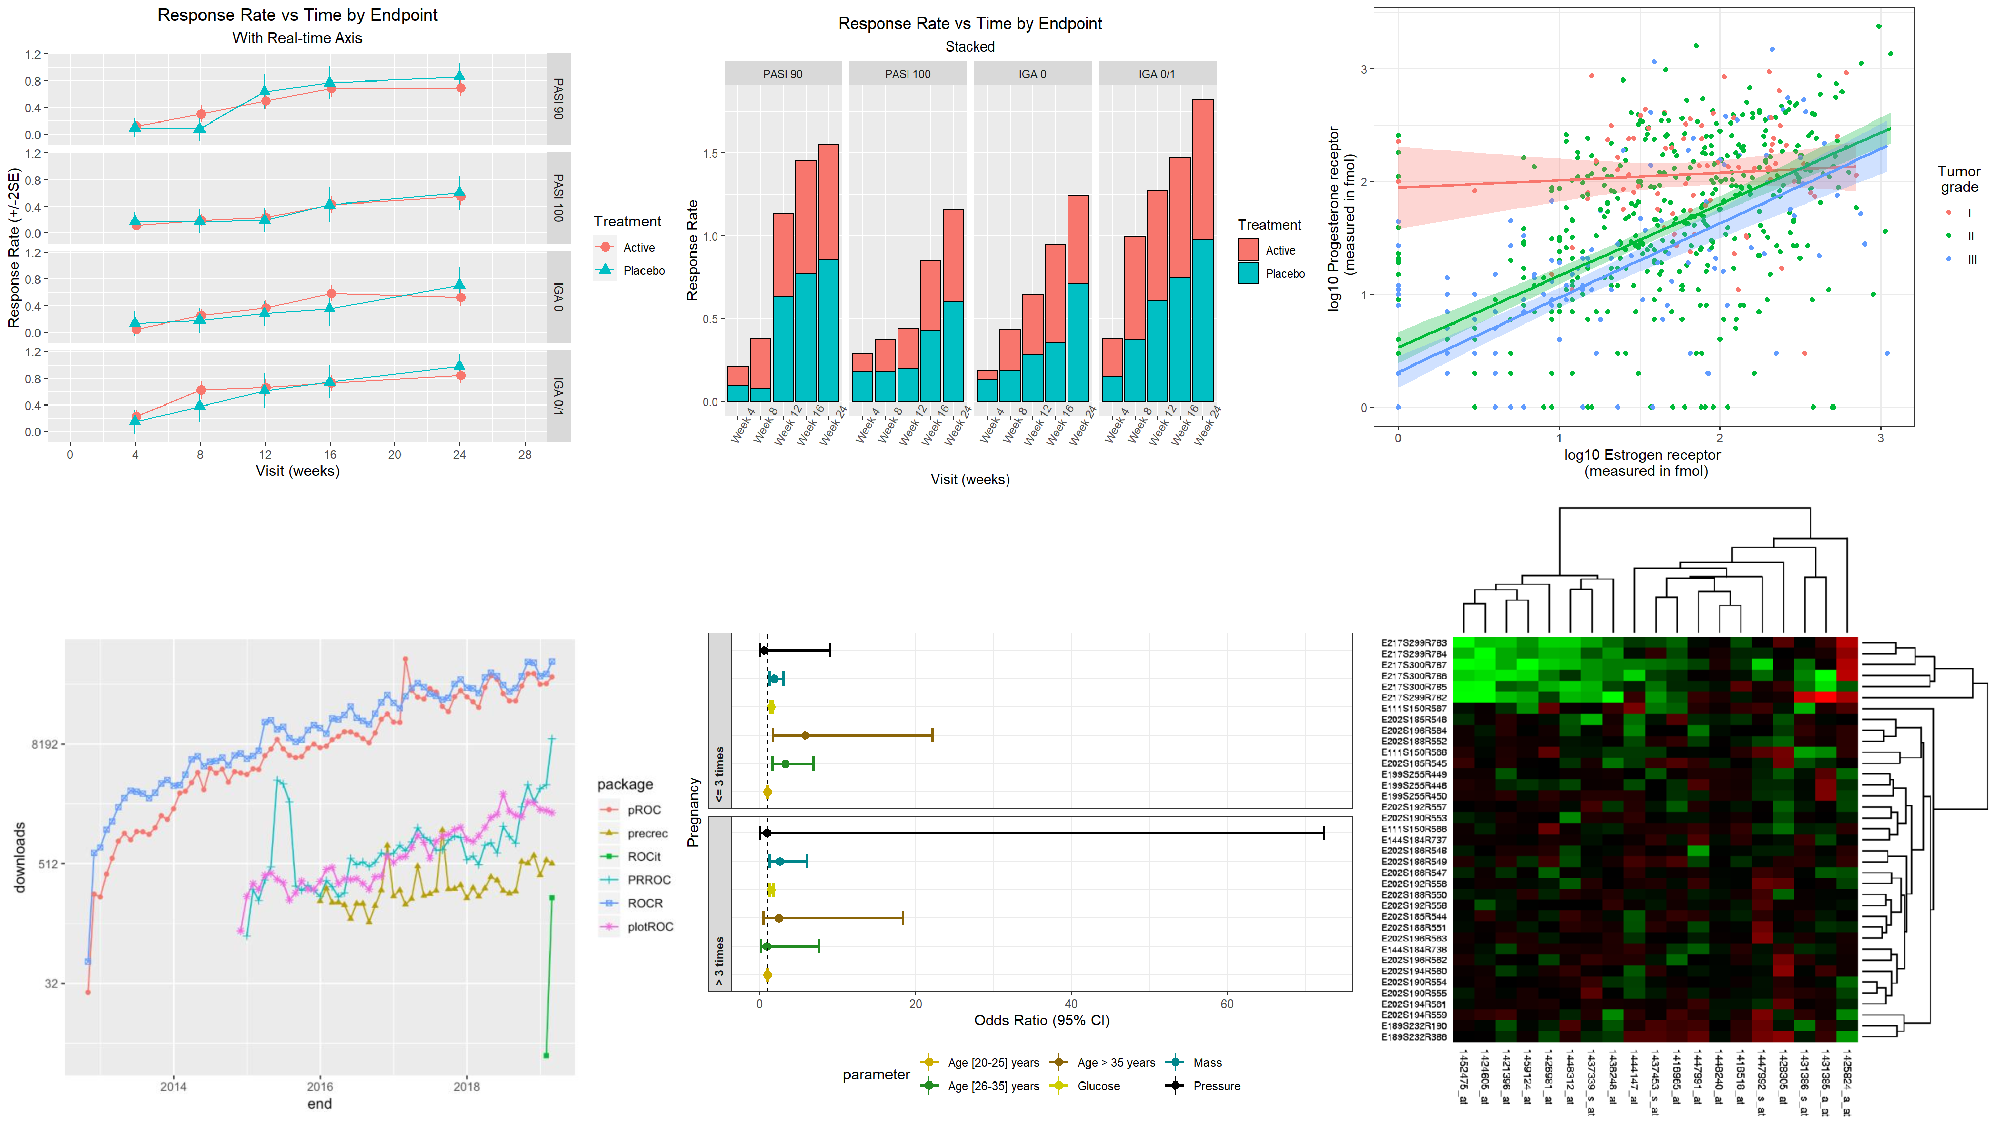
\includegraphics{figures/picCollage.pdf}}
  \caption{Showcasing different examples from the course.}
  \label{figure:picCollage}
\end{figure}

As a specific example, let us discuss the first assignment and its
possible solutions. Many assignments were kept open to interpretation of
the participants as we wanted to motivate everyone to come up with their
own solutions, rather than trying to follow one particular approach to
solve the assignment.

\noindent \textbf{Assignment 1}

\noindent \textbf{Data}

This data is taken from the R package \texttt{TH.data} \citep{Hothorn}.
For the data frame object GBSG2, there were 686 observations of the
following 10 variables:

\begin{itemize}
\tightlist
\item
  horTh: Hormonal therapy, a factor at two levels no and yes
\item
  age: Age of the patients in years
\item
  menostat: Menopausal status, a factor at two levels pre
  (premenopausal) and post (postmenopausal).
\item
  tsize: Tumor size (in mm)
\item
  tgrade: Tumor grade, a ordered factor at levels I \textless{} II
  \textless{} III.
\item
  pnodes: Number of positive nodes.
\item
  progrec: Progesterone receptor (in fmol).
\item
  estrec: Estrogen receptor (in fmol).
\item
  time: Recurrence free survival time (in days)
\item
  cens: Censoring indicator (0- censored, 1- event)
\end{itemize}

\noindent \textbf{Question}

Associated data was provided in an Excel file (Assign1.xlsx) and
participants were asked to solve the following questions:

\begin{itemize}
\tightlist
\item
  Produce a scatterplot for progesterone receptor (in fmol) vs.~estrogen
  receptor (in fmol). Add color and shape to include information on

  \begin{itemize}
  \tightlist
  \item
    Tumor Grade
  \item
    Menopausal Status
  \end{itemize}
\item
  Produce pairwise plots of progesterone receptor (in fmol) vs.~estrogen
  receptor (in fmol) vs.~tumor size. It should include additional
  information through color and shape to provide better understanding of
  data.
\end{itemize}

\noindent \textbf{Solution}

As the variable distributions were skewed, new variables were created
using the log transformation. There were also 0 values present which
required a basic scoring rule where 0 values were replaced by 1.

Solutions from different teams generally fell along the following 2
ways:

\begin{itemize}
\item
  Plot original data but the scale will be log-scale (Figure 5).
\item
  Plot the log-transformed data (Figure 6).
\item
  \texttt{ggpairs()} function was used to create the pairwise plot of
  the three variables as specified in the last part of the assignment
  (Figure 7).
\end{itemize}

\begin{Schunk}
\begin{figure}[h]

{\centering \includegraphics[width=0.8\linewidth]{paper_files/figure-latex/hw1plot1-1} 

}

\caption[Scatterplot for progesterone receptor (in fmol) vs]{Scatterplot for progesterone receptor (in fmol) vs. estrogen receptor (in fmol) in log-scale. Tumor grade and menopausal status are differentiated by the color and shape, respectively.}\label{fig:hw1plot1}
\end{figure}
\end{Schunk}

\begin{Schunk}
\begin{figure}[h]

{\centering \includegraphics[width=0.8\linewidth]{paper_files/figure-latex/hw1plot2-1} 

}

\caption[Scatterplot for log-transformed progesterone receptor (in fmol) vs]{Scatterplot for log-transformed progesterone receptor (in fmol) vs. log-transformed estrogen receptor (in fmol). Tumor grade and menopausal status are differentiated by the color and shape, respectively.}\label{fig:hw1plot2}
\end{figure}
\end{Schunk}

\begin{Schunk}
\begin{figure}[h]

{\centering \includegraphics[width=0.9\linewidth]{paper_files/figure-latex/hw1plot3-1} 

}

\caption[Pairwise Scatterplot of Progesterone, Estrogen and Tumor Size]{Pairwise Scatterplot of Progesterone, Estrogen and Tumor Size. Tumor grade and menopausal status are differentiated by the color and shape, respectively.}\label{fig:hw1plot3}
\end{figure}
\end{Schunk}

\hypertarget{how-to-crowdsource}{%
\subsubsection{How to crowdsource?}\label{how-to-crowdsource}}

RStudio Cloud was used as the primary platform during the entire course
of the training. In the beginning, we encountered some challenges with
the initial set up as we were using the Beta version of the RStudio
Cloud platform (the production environment was not available at that
time). RStudio team was prompt to resolve these issues by opening some
of the features such as the number of workspaces and projects per
account. As a starting point, we set up different workspaces for
different TAs and RStudio engineers helped us configure those workspaces
properly. The \texttt{assignment} feature of RStudio Cloud helped us to
easily distribute the assignments for all the workspaces. Different
features available for RStudio Cloud are discussed in the next
subsection.

\vspace{0.35cm}

\noindent \textbf{About RStudio Cloud}

RStudio Cloud is a hosted version of RStudio in the cloud. It is
maintained by RStudio and has a nice web interface together with certain
features which made it the most suitable option for us.

\begin{figure}[htbp]
  \centering
  \scalebox{0.23}{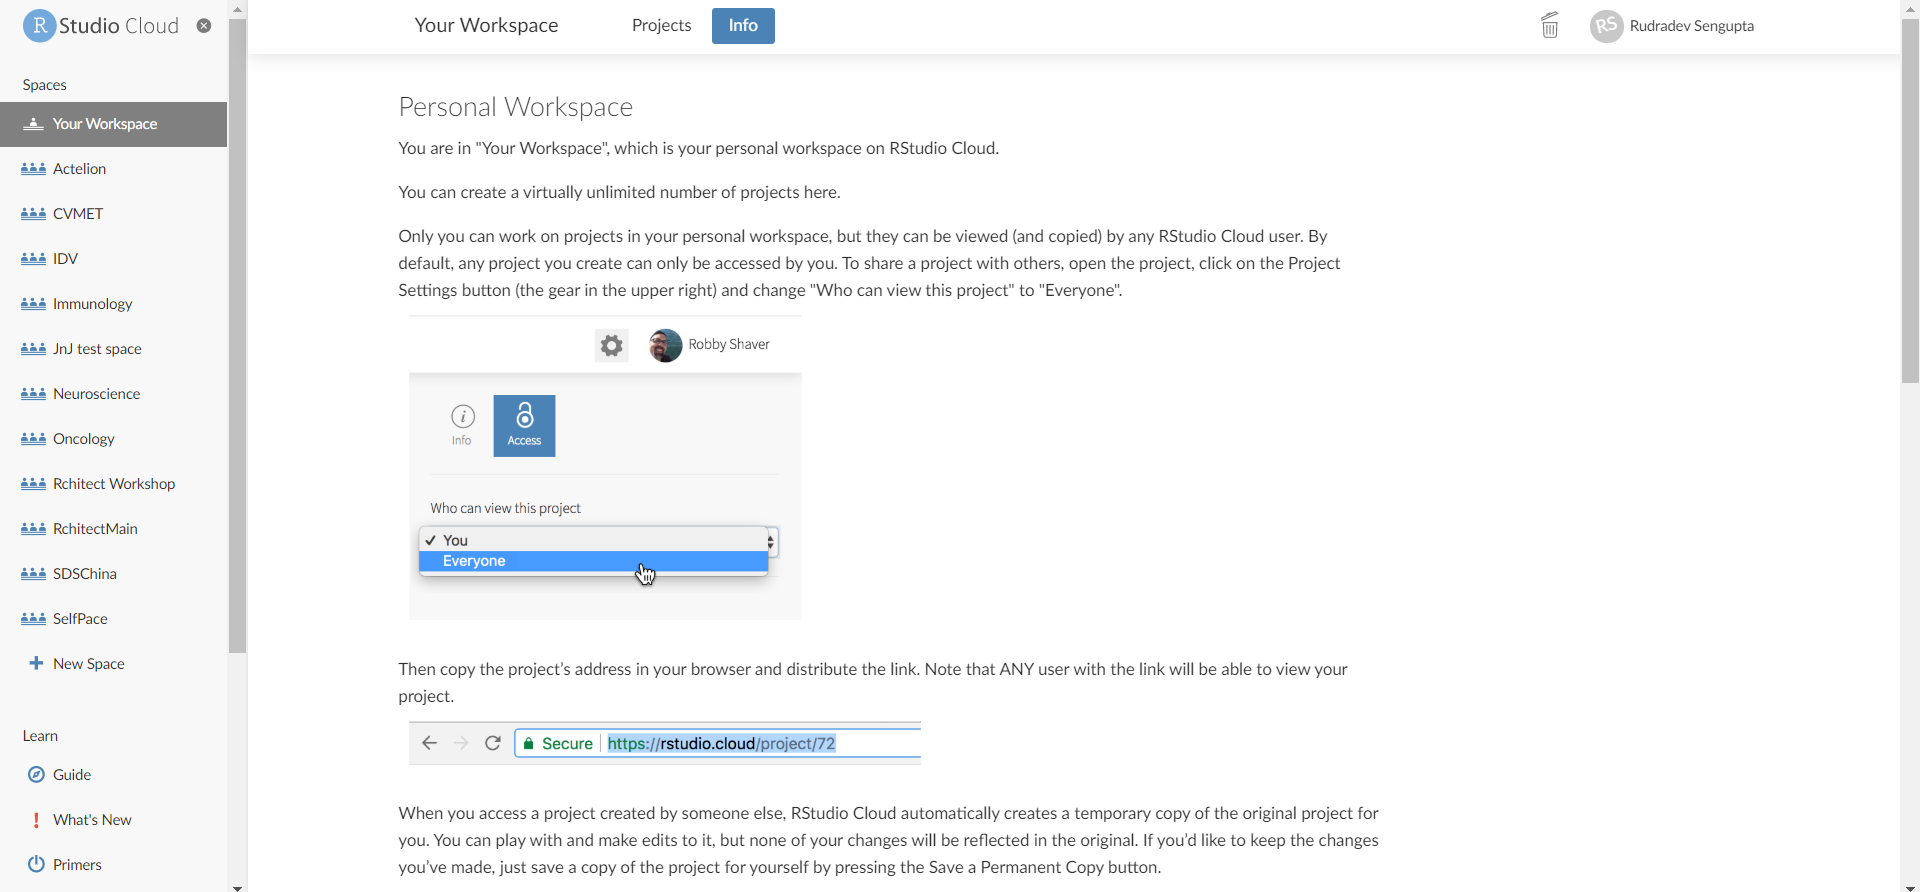
\includegraphics{figures/RStudioCloudOverview}}
  \caption{Overview of RStudio Cloud.}
  \label{figure:rscloud}
\end{figure}

Many organizations are embarking on data science educational initiatives
and academies to help bring employees up to speed on state of the art
analytical topics. RStudio Cloud is a hosted version of RStudio that
continues the mission and dedication to a sustainable investment in free
and open-source software for data science, scientific research,
education, and technical communication. RStudio Cloud makes it easy for
anyone to do, share, teach, and learn data science, by allowing students
and instructors to:

\begin{itemize}
\tightlist
\item
  Analyze data using the RStudio IDE directly from a browser
\item
  Share projects and analysis with teams, classrooms, workshops, or the
  world
\item
  Use interactive tutorials and primers to learn the basics of data
  science
\item
  No hardware, configuration, or installation required
\end{itemize}

One of the most effective ways to get started learning R is to start
using it. RStudio Cloud is designed to make educational data science
efforts easier for instructors and students by removing complicated
setup and environment configuration. Projects are the fundamental unit
of work on RStudio Cloud - projects encapsulate R code, packages and
data files and provide isolation from other analyses or course work.
Projects can be public or private and are created and managed from a
user's workspace. Public projects can allow people to interact with an
analysis by visiting a shared link. Every RStudio Cloud user gets a
personal workspace in which to create projects. Users can also create
private, shared spaces that function as virtual classrooms for courses
and workshops. Users who can access a specific workspace can be assigned
different roles, giving them capabilities appropriate for instructors,
teaching assistants and students.

When an instructor is teaching a class or workshop, RStudio projects can
be made into assignments and academic content for students. Students can
work on the assignments and instructors can assess their work and check
progress. Students can also make copies of class projects created by the
instructor, with the necessary environment and packages automatically
replicated. Instructors can access usage metrics for any shared space
where they are an admin or moderator. They can view summary information
for the space, and data for individual members and their projects.
Summary metrics include total project hours and the number of active
spaces, members, and projects. These integrations mean that instructors
do not need to spend time managing environments or troubleshooting
student technical issues. Instructors can focus on what is most
important - teaching data science.

\noindent \textbf{Setting up RStudio Cloud}

Six separate workspaces were set up for five different TAs and one
specifically for the China region. The ``Assignment'' feature of RStudio
Cloud was used to post the assignments in every workspace from GitHub.
This feature helped the participants to easily create their own copies
of the assignments and then work on it on their own time. Initially, the
``Base Project'' feature was used to control the package management so
that the beginners can directly start working on the assignments without
worrying about R package installation. Later participants were
encouraged to install the packages on their own to get more familiar
with R

\noindent \textbf{Assignment workflow}

At week 0, the first assignment was posted in all the six workspaces in
RStudio Cloud and all the participants were notified so they could start
working on the assignments as soon as they were ready. Then the group
leaders organized TA status review sessions during week 1 to discuss the
assignment within the corresponding groups. One colleague from each TA
would be selected to present the solution on behalf of the group, in the
regroup session happening at week 2. The status review sessions also
helped the group members that stayed behind, either due to difficulties
understanding/performing the task or due to lack of time because of
daily projects, to catch up. During the regroup sessions in week 2 all
groups presented their solutions, and discussion on the different
approaches helped all participants learn more about other tools and
approaches within R. One ``tips and tricks'' presentation, with examples
on R-based graphics in everyday work, was hosted during these regroup
sessions to showcase how R can help us visualize and explore
pharmaceutical data as well as showcase advanced R programming
techniques. Also, during the regroup sessions some hints and background
information for the next assignment were discussed. After every regroup
session the recorded videos and the solutions by all groups were made
available through standard sharing platforms. The next assignment was
than made available in RStudio Cloud within 24 hours and everyone was
notified. This iterative biweekly process was used for all 16
assignments over 8 months. Besides, the regular workflow as displayed in
Figure \ref{figure_workflow}, different subgroups hosted their
within-group sessions as per requirements.

\begin{figure}[htbp]
  \centering
  \scalebox{0.35}{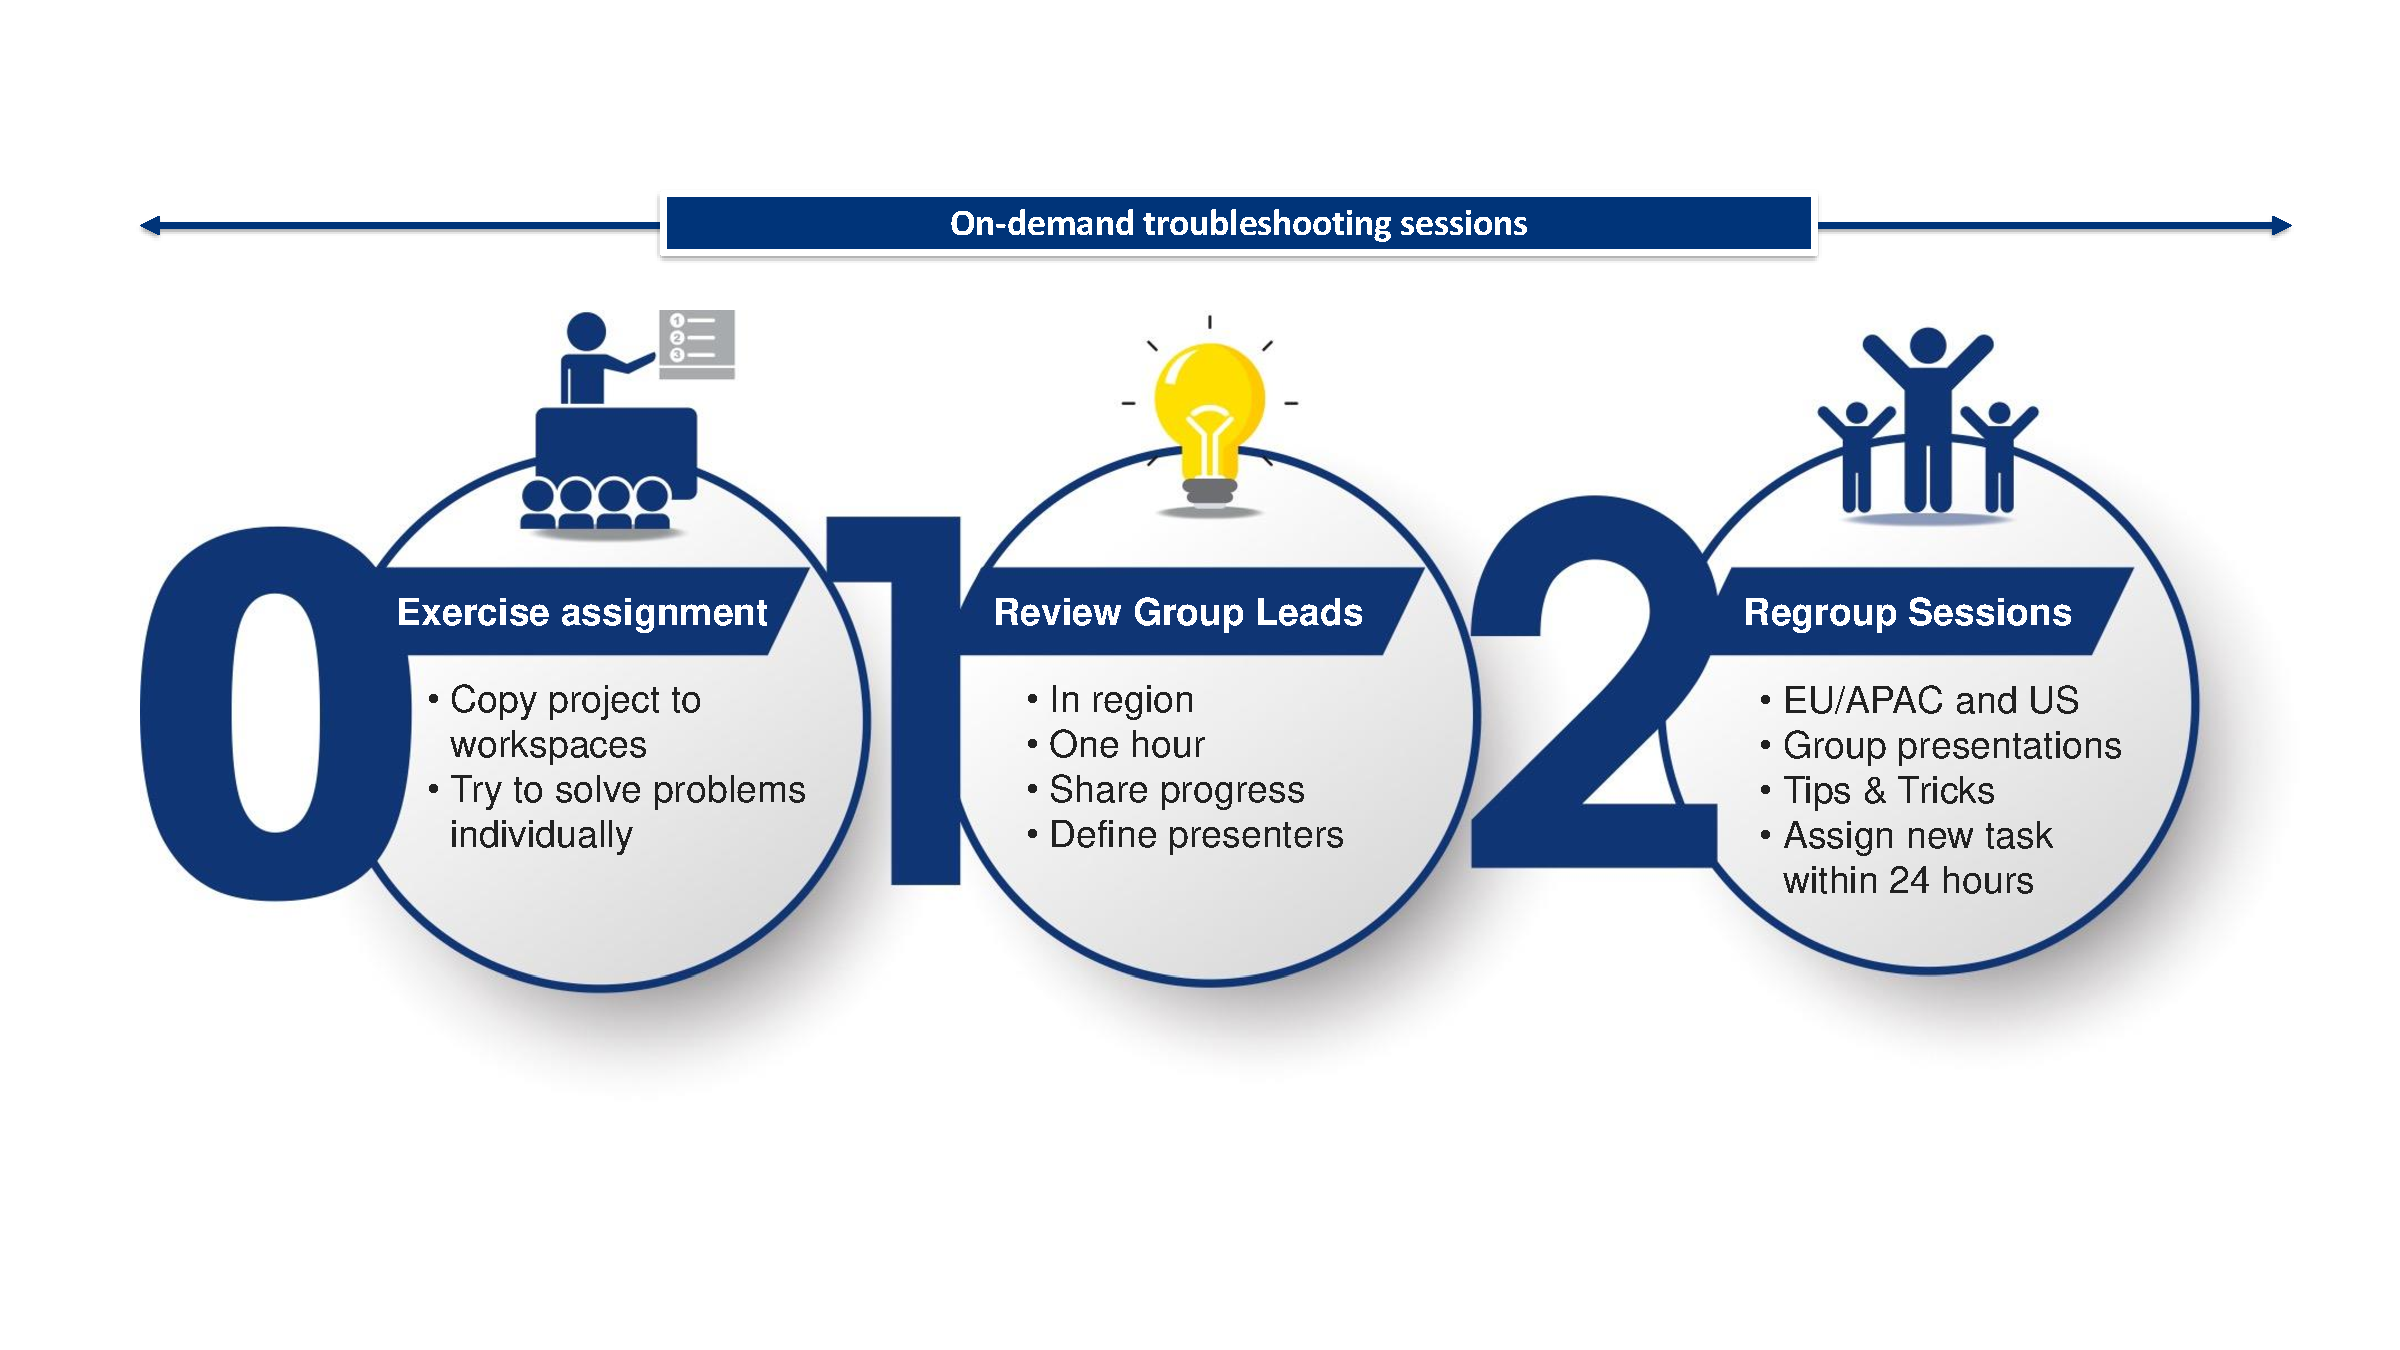
\includegraphics{figures/biweekly.pdf}}
  \caption{Bi-weekly approach for the assignments.}
  \label{figure_workflow}
\end{figure}

\hypertarget{project-metrics}{%
\subsection{Project metrics}\label{project-metrics}}

The training started with a virtual kick-off meeting where the
objectives and the format of the course was laid out. More than 200
people attended the kick-off meeting as it was a group-wide initiative.
The first assignment had 170 participants. However, that participation
quickly dropped to between 100 to 120 participants per week by the time
the third assignment was handed out and this number held steady until
the end of the training.

A second survey was sent to the participants at the conclusion of the
training and was completed by about half (N=56) of the cohort that
participated until the end. About 40\% of the respondents had never used
R and after the training 36\% felt they managed to achieve a beginners'
level proficiency in R. Of that 36\% indicating proficiency, 50\% were
at intermediate level and 13\% at advanced level. 63\% of the
respondents said they participated on all or almost all the sessions. A
little over 50\% thought the assignments were challenging. All but 2
respondents thought the training was a valuable use of their time and 3
said they would not like to continue learning R. One third of the
respondents said they are now using R in their day-to-day activities. We
also questioned how much time they spent on average every week to
complete the assignments. 43\% spent at most a couple of hours, whereas
34\% had to work for 2-4 hours, and 13\% worked for more than 4 hours
every week to finish the assignments.

\hypertarget{management-perspective}{%
\subsection{Management perspective}\label{management-perspective}}

The Graphics with R initiative was generated from a high-level goal of
the head and senior leadership team of the entire statistician
organization within the Janssen R \& D subsidiary of Johnson \& Johnson.
The umbrella strategic goal was centered on leveraging new technologies
to build our capabilities to add value in alignment with mission
components of driving robust and scientifically informed decision-making
to discover and develop medicines for patients in need. Raising the
organization's collective competency in graphics, using the software
environment R, was settled upon as an achievable and concrete target. A
charter was developed. A quantitative metric was set to reach at least
75\% participation and proficiency across more than 200 clinical
statisticians in the community. Messaging was clear from the very top
leadership of the statistics organization that creating graphics with R
was a required objective for everyone.

It was especially gratifying how broadly the statistics community took
this charter and its principles. The entire community was willing to
iterate and continuously get better individually via crowdsourcing. They
obtained the necessary skills, predominantly through (1) self learning
with online resources and (2) working with colleagues in a collaborative
manner. There were multiple cases of colleagues, from early through
later stages of their careers, who had no prior knowledge of R, yet
surprised themselves in learning how to efficiently develop and
successfully display visualizations, often within the 2 weeks period
between assignments described earlier. This had substantial side
benefits for raising other collective competencies of reporting, data
wrangling, and coding across the organization.

By the second assignment presentation, the core oversight team decided
that \texttt{ggplot} would be required as the sole system within R to
fulfill the remaining assignments. Similarly, by the fourth assignment
presentation, R Markdown or the RStudio IDE was required by the core
team for all participants. These midstream iterations were generally
well-received and followed by participants. The core team had
communicated at the start of the series that such iterations were likely
as the crowdsourcing framework was being used for the first time within
the organization.

One high performer even took the opportunity to apply their new graphics
and R skills to an ongoing real-time health authority dialogue. A
visualization helped persuade agreement on use of a biomarker for more
accurate prediction of survival in cancer patients.

Ongoing next steps are to broaden the use of graphics with R and R
Markdown for rapid delivery of topline reports (TLR). TLRs are important
channels for top executive reviews and decisions of the truly critical
statistical results after the completion of clinical trials.

\hypertarget{summary-and-discussion}{%
\subsection{Summary and discussion}\label{summary-and-discussion}}

RStudio Cloud was an excellent tool to introduce the participants to R
and manage the distribution of the exercises as well as capture
essential metrics on the engagement. We did not need to worry about R
installations or access permissions to internal cloud resources as
RStudio Cloud already took care of these details inherently. Also, by
distributing the exercises through the RStudio Cloud project we could
seamlessly include all dependencies, such as packages, with the
necessary instructions to complete the work.

As the program was designed with great flexibility there were important
lessons, learnt throughout the journey, which were continuously used as
feedback to improve the program. The set up of the exercises without the
obligation of producing a specific outcome provided different teams an
opportunity to create diverse solutions on how to achieve the end
results. For instance, the initial focus of the training was the
creation of graphics using R but as the training developed some groups
introduced the use of RMarkdown to complete the exercise, and after
exposing the entire group to this new tool and the use of one of the
tips and tricks sessions to delve into the technology, all the groups
were able to implement this new aspect of the training. Another examples
of this diversity was the introduction of R packages beyond those
installed in RStudio Cloud for the completion of the exercises. The same
flexibility caused some discomfort to some of the participants,
particularly in the beginning of the training. However, we managed to
overcome this challenge via the tips and tricks sessions as well as by
providing hints for certain questions of the assignments. It is also
important to highlight that although we maintained great flexibility
throughout the course, adapting as we moved along, the project started
with a great deal of planning where discussions with all volunteers
helped craft the proper curriculum that catered to the diverse needs of
all TAs, as different graphics are commonly used in their daily work.
Moreover, there was a huge background effort to identify and define the
best platform (RStudio Cloud) to be used during the course for
programming and sharing the information.

Although strongly encouraged by upper management this training was
non-mandatory therefore we believe that overall the training was
successful as a participation rate between 60\%-70\% (from initial
dates) was maintained. Besides the strong participation another key
metric for success was the fact that a third of the users was using what
they learnt on their daily jobs after the conclusion of the training.
Part of this success can be attributed to the design of the training as
participants engaged on the assignments every week for an extended
period of time therefore becoming more comfortable with the use of the
language. This certainly helped with retaining knowledge.

From the management perspective the Graphics with R initiative proved to
be an efficient method to train a large group of colleagues with minimal
disruption on the daily operations of the group. The crowdsourcing
format was crucial as learners took ownership on their learning and
dedicated themselves at their own pace. Beyond the actual advancement of
programming skills the opportunity to develop soft skills was also
greatly appreciated by the management team and was evident in raising
the broad collective capabilities on communication skills. Due to this
success two other training initiatives adapted crowdsourcing methods and
were implemented. Therefore we believe crowdsourcing is a powerful
method for modern training in the professional setting.

\hypertarget{acknowledgement}{%
\subsection{Acknowledgement}\label{acknowledgement}}

We would like to acknowledge all the volunteers who agreed to help us
out during this journey in various means e.g., by creating the
assignments, by presenting during tips and tricks sessions, by helping
their colleagues with one-one sessions to help them improve, etc.
Janssen colleagues who were invaluable to this initiative: Katleen
Callewaert, Yannick Vandendijck, Beatriz Lopez Sanchez, Etienne Ernault,
Monelle Tamegnon, Lixia Pei, Cynthia Gargano, Jianfeng Xu, Bin Gao,
Xiang Li, Iva Kezic, Xin Qiu, Sabrina El Bachiri, Yan Liu, Xiaoming Li,
Jinxiang Wu, Weiping Liu, Stefan Avey, Volha Tryputsen, Martin Otava,
Davit Sargsyan, Ewoud de Troyer, Jocelyn Sendecki, Oluyemi Oyeniran,
Marjolein Crabbe, Leacky Muchene, Jan Serroyen, Jeroen Tolboom, Leen
Slaets, Sumesh Kalappurakal and Axel Muehlig. We also want to thank
Robby Shaver from RStudio for his invaluable support with the RStudio
Cloud platform.

\bibliography{RJreferences}


\address{%
Rudradev Sengupta\\
Johnson \& Johnson\\
Turnhoutseweg 30, 2340 Beerse, Belgium\\
}
\href{mailto:rsengup4@its.jnj.com}{\nolinkurl{rsengup4@its.jnj.com}}

\address{%
Paulo R. Bargo\\
Johnson \& Johnson\\
Spring House, PA 19477, United States\\
}
\href{mailto:pbargo@its.jnj.com}{\nolinkurl{pbargo@its.jnj.com}}

\address{%
Bill Pikounis\\
Johnson \& Johnson\\
Spring House, PA 19477, United States\\
}
\href{mailto:bpikounis@its.jnj.com}{\nolinkurl{bpikounis@its.jnj.com}}

\address{%
Surya Mohanty\\
Johnson \& Johnson\\
Spring House, PA 19477, United States\\
}
\href{mailto:smohanty@its.jnj.com}{\nolinkurl{smohanty@its.jnj.com}}

\address{%
Jason Milnes\\
RStudio, PBC\\
Pittsburgh, PA, United States\\
}
\href{mailto:Jason@rstudio.com}{\nolinkurl{Jason@rstudio.com}}

\address{%
Philip Bowsher\\
RStudio, PBC\\
Pittsburgh, PA, United States\\
}
\href{mailto:Phil@rstudio.com}{\nolinkurl{Phil@rstudio.com}}

